
%% bare_conf.tex
%% V1.4b
%% 2015/08/26
%% by Michael Shell
%% See:
%% http://www.michaelshell.org/
%% for current contact information.
%%
%% This is a skeleton file demonstrating the use of IEEEtran.cls
%% (requires IEEEtran.cls version 1.8b or later) with an IEEE
%% conference paper.
%%
%% Support sites:
%% http://www.michaelshell.org/tex/ieeetran/
%% http://www.ctan.org/pkg/ieeetran
%% and
%% http://www.ieee.org/

%%*************************************************************************
%% Legal Notice:
%% This code is offered as-is without any warranty either expressed or
%% implied; without even the implied warranty of MERCHANTABILITY or
%% FITNESS FOR A PARTICULAR PURPOSE! 
%% User assumes all risk.
%% In no event shall the IEEE or any contributor to this code be liable for
%% any damages or losses, including, but not limited to, incidental,
%% consequential, or any other damages, resulting from the use or misuse
%% of any information contained here.
%%
%% All comments are the opinions of their respective authors and are not
%% necessarily endorsed by the IEEE.
%%
%% This work is distributed under the LaTeX Project Public License (LPPL)
%% ( http://www.latex-project.org/ ) version 1.3, and may be freely used,
%% distributed and modified. A copy of the LPPL, version 1.3, is included
%% in the base LaTeX documentation of all distributions of LaTeX released
%% 2003/12/01 or later.
%% Retain all contribution notices and credits.
%% ** Modified files should be clearly indicated as such, including  **
%% ** renaming them and changing author support contact information. **
%%*************************************************************************


% *** Authors should verify (and, if needed, correct) their LaTeX system  ***
% *** with the testflow diagnostic prior to trusting their LaTeX platform ***
% *** with production work. The IEEE's font choices and paper sizes can   ***
% *** trigger bugs that do not appear when using other class files.       ***                          ***
% The testflow support page is at:
% http://www.michaelshell.org/tex/testflow/

\documentclass[12pt,twoside,a4paper,openright]{report}
\usepackage{etex}
% Select encoding of your inputs.
\usepackage[utf8]{inputenc}

% Make latex understand and use the typographic
% rules of the language used in the document.
\usepackage[english, danish]{babel}

% Use the vector font Latin Modern which is going
% to be the default font in latex in the future.
\usepackage{lmodern}

% Choose the font encoding
\usepackage[T1]{fontenc}

% Use colour in tables
\usepackage[table]{xcolor}
\usepackage{array}
\usepackage{multirow}

% load a colour package
\usepackage{xcolor}
\definecolor{aaublue}{RGB}{33,26,82}% dark blue

% The standard graphics inclusion package
\definecolor{white}{RGB}{255,255,255} % define color white
\usepackage{graphicx}
\usepackage{adjustbox}

% Set up how figure and table captions are displayed
\usepackage{caption}
\captionsetup{
  font=footnotesize,% set font size to footnotesize
  labelfont=bf % bold label (e.g., Figure 3.2) font
}

% Enable row combination in tables
\usepackage{multirow}

% Make space between table lines and text
\renewcommand{\arraystretch}{1.5}

% Make the standard latex tables look so much better
\usepackage{array,booktabs}

% Enable the use of frames around, e.g., theorems
% The framed package is used in the example environment
\usepackage{framed}
\usepackage{colortbl}
\usepackage{longtable}
\usepackage{xcolor}
\usepackage{textcomp}

%%%%%%%%%%%%%%%%%%%%%%%%%%%%%%%%%%%%%%%%%%%%%%%%
% Mathematics
%%%%%%%%%%%%%%%%%%%%%%%%%%%%%%%%%%%%%%%%%%%%%%%%
% Defines new environments such as equation,
% align and split 
\usepackage{amsmath}
\usepackage{relsize}
% Adds new math symbols
\usepackage{amssymb}
% Use theorems in your document
% The ntheorem package is also used for the example environment
% When using thmmarks, amsmath must be an option as well. Otherwise \eqref doesn't work anymore.
\usepackage[framed,amsmath,thmmarks]{ntheorem}
\usepackage{cancel}

%%%%%%%%%%%%%%%%%%%%%%%%%%%%%%%%%%%%%%%%%%%%%%%%
% Page Layout
%%%%%%%%%%%%%%%%%%%%%%%%%%%%%%%%%%%%%%%%%%%%%%%%
% Change margins, papersize, etc of the document
\usepackage[
  left=25mm,% left margin on an odd page %tidligere 25mm for baade right og left
  right=25mm,% right margin on an odd page
  top=35mm,
  ]{geometry}
  
% Modify how \chapter, \section, etc. look
% The titlesec package is very configureable
\usepackage{titlesec}
\makeatletter
\def\ttl@mkchap@i#1#2#3#4#5#6#7{%
    \ttl@assign\@tempskipa#3\relax\beforetitleunit
    \vspace{\@tempskipa}%<<<<<< REMOVE THE * AFTER \vspace
    \global\@afterindenttrue
    \ifcase#5 \global\@afterindentfalse\fi
    \ttl@assign\@tempskipb#4\relax\aftertitleunit
    \ttl@topmode{\@tempskipb}{%
        \ttl@select{#6}{#1}{#2}{#7}}%
    \ttl@finmarks  % Outside the box!
    \@ifundefined{ttlp@#6}{}{\ttlp@write{#6}}}
\makeatother

\titlespacing{\chapter}{0pt}{0pt}{10pt}
\titlespacing{\section}{0pt}{0pt}{-5pt}
\titlespacing{\subsection}{0pt}{8pt}{-5pt}
\titlespacing{\subsubsection}{0pt}{6pt}{-10pt}

\titleformat*{\section}{\normalfont\Large\bfseries\color{aaublue}}
\titleformat*{\subsection}{\normalfont\large\bfseries\color{aaublue}}
\titleformat*{\subsubsection}{\normalfont\normalsize\bfseries\color{aaublue}}

\usepackage{bookmark}
\usepackage{titlesec, blindtext, color}
%\color{gray75}{gray}{0.75}
\newcommand{\hsp}{\hspace{20pt}}
\titleformat{\chapter}[hang]{\Huge\bfseries}{\thechapter\hsp\textcolor{aaublue}{|}\hsp}{0pt}{\Huge\bfseries}

% Change the headers and footers
\usepackage{fancyhdr}
\setlength{\headheight}{15pt}
\pagestyle{fancy}
\fancyhf{} %delete everything
\renewcommand{\headrulewidth}{0pt} %remove the horizontal line in the header
\fancyhead[RO,LE]{\color{aaublue}\small\nouppercase\leftmark} %even page - chapter title
\fancyhead[LO]{}
\fancyhead[RE]{} 
\fancyhead[CE]{}
\fancyhead[CO]{}
\fancyfoot[RE,LO]{\thepage}
\fancyfoot[LE,RO]{} %page number on all pages
\fancyfoot[CE,CO]{}

% change first page of all chapters header and footer to fancy style
\makeatletter
\let\ps@plain\ps@fancy
\makeatother

% Do not stretch the content of a page. Instead,
% insert white space at the bottom of the page
\raggedbottom

% Enable arithmetics with length. Useful when typesetting the layout.
\usepackage{calc}

%%%%%%%%%%%%%%%%%%%%%%%%%%%%%%%%%%%%%%%%%%%%%%%%
% Bibliography
%%%%%%%%%%%%%%%%%%%%%%%%%%%%%%%%%%%%%%%%%%%%%%%%
%setting references (using numbers) and supporting i.a. Chicargo-style:
\usepackage{etex}
\usepackage{etoolbox}
\usepackage{keyval}
\usepackage{ifthen}
\usepackage{url}
\usepackage{csquotes}
\usepackage[backend=biber, url=true, doi=true, style=numeric, sorting=none]{biblatex}
\addbibresource{setup/bibliography.bib}

%%%%%%%%%%%%%%%%%%%%%%%%%%%%%%%%%%%%%%%%%%%%%%%%
% Misc
%%%%%%%%%%%%%%%%%%%%%%%%%%%%%%%%%%%%%%%%%%%%%%%%

%%% Enables the use FiXme refferences. Syntax: \fxnote{...} %%%
\usepackage[footnote, draft, english, silent, nomargin]{fixme}
%With "final" instead of "draft" an error will ocure for every FiXme under compilation.

%%% allows use of lorem ipsum (generate i.e. pagagraph 1 to 5 with \lipsum[1-5]) %%%
\usepackage{lipsum}

%%% Enables figures with text wrapped tightly around it %%%
\usepackage{wrapfig}

%%% Section debth included in table of contents (1 = down to sections) %%%
\setcounter{tocdepth}{1}

%%% Section debth for numbers (1 = down to sections) %%%
\setcounter{secnumdepth}{1}

\usepackage{tocloft}
\setlength{\cftbeforetoctitleskip}{0 cm}
\renewcommand{\cftpartpresnum}{Part~}
\let\cftoldpartfont\cftpartfont
\renewcommand{\cftpartfont}{\cftoldpartfont\cftpartpresnum}

%%%%%%%%%%%%%%%%%%%%%%%%%%%%%%%%%%%%%%%%%%%%%%%%
% Hyperlinks
%%%%%%%%%%%%%%%%%%%%%%%%%%%%%%%%%%%%%%%%%%%%%%%%

% Enable hyperlinks and insert info into the pdf
% file. Hypperref should be loaded as one of the 
% last packages
\usepackage{nameref}
\usepackage{hyperref}
\hypersetup{%
	%pdfpagelabels=true,%
	plainpages=false,%
	pdfauthor={Author(s)},%
	pdftitle={Title},%
	pdfsubject={Subject},%
	bookmarksnumbered=true,%
	colorlinks,%
	citecolor=aaublue,%
	filecolor=aaublue,%
	linkcolor=aaublue,% you should probably change this to black before printing
	urlcolor=aaublue,%
	pdfstartview=FitH%
}

% remove all indentations
\setlength\parindent{0pt}
\parskip 5mm
\usepackage{verbatim}

\definecolor{Gra}{RGB}{230,230,230}

%creates a nice-looking C#-text
\newcommand{\CC}{C\nolinebreak\hspace{-.05em}\raisebox{.3ex}{\scriptsize\text \#} }

%enables multi column lists
\usepackage{multicol}

%enables code-examples
\usepackage{listings}

\definecolor{coolblue}{RGB}{32,95,128}
\definecolor{mygreen}{rgb}{0,0.6,0}
\definecolor{mygray}{rgb}{0.5,0.5,0.5}
\definecolor{mymauve}{rgb}{0.58,0,0.82}
\usepackage{textcomp}
\definecolor{listinggray}{gray}{0.9}
\definecolor{lbcolor}{rgb}{0.9,0.9,0.9}

\lstdefinestyle{customcpp}{
    backgroundcolor=\color{lbcolor},
    tabsize=4,
    rulecolor=,
    language=C++,
    basicstyle=\scriptsize,
    upquote=true,
    aboveskip={1.5\baselineskip},
    columns=fixed,
    showstringspaces=false,
    extendedchars=true,
    breaklines=true,
    prebreak = \raisebox{0ex}[0ex][0ex]{\ensuremath{\hookleftarrow}},
    frame=single,
    showtabs=false,
    numbers=left,
    captionpos=b,
    numbersep=5pt,
    numberstyle=\tiny\color{mygray},
    showspaces=false,
    showstringspaces=false,
    identifierstyle=\ttfamily,
    keywordstyle=\color[rgb]{0,0,1},
    commentstyle=\color[rgb]{0.133,0.545,0.133},
    stringstyle=\color[rgb]{0.627,0.126,0.941},
}
\lstdefinestyle{custommatlab}{
    backgroundcolor=\color{lbcolor},
    tabsize=4,
    rulecolor=,
    language=Matlab,
    basicstyle=\scriptsize,
    upquote=true,
    aboveskip={1.5\baselineskip},
    columns=fixed,
    showstringspaces=false,
    extendedchars=true,
    breaklines=true,
    prebreak = \raisebox{0ex}[0ex][0ex]{\ensuremath{\hookleftarrow}},
    frame=single,
    showtabs=false,
    numbers=left,
    captionpos=b,
    numbersep=5pt,
    numberstyle=\tiny\color{mygray},
    showspaces=false,
    showstringspaces=false,
    identifierstyle=\ttfamily,
    keywordstyle=\color[rgb]{0,0,1},
    commentstyle=\color[rgb]{0.133,0.545,0.133},
    stringstyle=\color[rgb]{0.627,0.126,0.941},   
}
\lstdefinestyle{custommatlabinline}{
    style=custommatlab,
    basicstyle=\small,
}
\lstdefinestyle{customcppinline}{
    style=customcpp,
    basicstyle=\small,
}
\lstset{
%  backgroundcolor=\color{white},   % choose the background color; you must add \usepackage{color} or \usepackage{xcolor}
%  basicstyle=\footnotesize,        % the size of the fonts that are used for the code
%  breakatwhitespace=false,         % sets if automatic breaks should only happen at whitespace
%  breaklines=true,                 % sets automatic line breaking
%  captionpos=t,                    % sets the caption-position to bottom
%  commentstyle=\color{mygreen},    % comment style
%  deletekeywords={...},            % if you want to delete keywords from the given language
%  escapeinside={\%*}{*)},          % if you want to add LaTeX within your code
%  extendedchars=true,              % lets you use non-ASCII characters; for 8-bits encodings only, does not work with UTF-8
%  frame=single,                    % adds a frame around the code
%  keepspaces=true,                 % keeps spaces in text, useful for keeping indentation of code (possibly needs columns=flexible)
%  keywordstyle=\color{blue},       % keyword style
%  language=C++,                 % the language of the code
%  morekeywords={*,...},            % if you want to add more keywords to the set
%  numbers=left,                    % where to put the line-numbers; possible values are (none, left, right)
%  numbersep=5pt,                   % how far the line-numbers are from the code
%  numberstyle=\tiny\color{mygray}, % the style that is used for the line-numbers
%  rulecolor=\color{black},         % if not set, the frame-color may be changed on line-breaks within not-black text (e.g. comments (green here))
%  showspaces=false,                % show spaces everywhere adding particular underscores; it overrides 'showstringspaces'
%  showstringspaces=false,          % underline spaces within strings only
%  showtabs=false,                  % show tabs within strings adding particular underscores
%  stepnumber=1,                    % the step between two line-numbers. If it's 1, each line will be numbered
%  stringstyle=\color{mymauve},     % string literal style
%  tabsize=2,                       % sets default tabsize to 2 spaces
%  title=\lstname                   % show the filename of files included with \lstinputlisting; also try caption instead of title
    style=customcpp
}

\usepackage{float}
\usepackage{caption}
\usepackage{subcaption}
\usepackage{siunitx}
\sisetup{decimalsymbol=comma}
\sisetup{detect-weight}

\usepackage{enumitem}
%\usepackage[citestyle=authoryear,natbib=true]{biblatex}

% Figures - TIKZ
\usepackage{tikz}
\usetikzlibrary{shapes,arrows}
\usepackage[americanresistors,americaninductors,americancurrents, americanvoltages]{circuitikz}

% Wall of text logo
\newcommand{\walloftextalert}[0]{\includegraphics[width=\textwidth]{walloftext.png}}

\usepackage{pdfpages}
\usepackage{lastpage}
\usepackage{epstopdf}

\setlength{\headheight}{21pt}

\hfuzz=\maxdimen
\tolerance = 10000
\hbadness  = 10000

\usepackage{siunitx}
\graphicspath{{./figures/}}% package inclusion and set up of the document

%%%%%%%%%%%%%%%%%%%%%%%%%%%%%%%%%%%%%%%%%%%%%%%%%%%%%
%             UNITS, EQUATIONS AND TEXT             %
%%%%%%%%%%%%%%%%%%%%%%%%%%%%%%%%%%%%%%%%%%%%%%%%%%%%%
%Units:
\newcommand{\unit}[1]{&& \left[\si{#1}\right]} %\newcommand{\unit}[1]{[\si{#1}]}             <<| Use these if you want equations to be
\newcommand{\unitWh}[1]{[\si{#1}]}             %\newcommand{\eq}[2]{&&\si{#1} &= \si{#2}&&}  <<| centered.. .. will appear scrambled
\newcommand{\numUnit}[1]{\ \si{#1}&}           %                                               | from one equation to the next though..
%Equation:                                     %                                               | and does not work with long equations.. :/
\newcommand{\eq}[2]{\si{#1} &= \si{#2}}
\newcommand{\arw}{&& &\Updownarrow&&}
\newcommand{\eqOne}[2]{\si{#1} &= \si{#2} &\nonumber\\}
\newcommand{\eqTwo}[1]{&\ \ \ \ \si{#1}&}
%Text:
\newcommand{\tx}[1]{\text{#1}}
%Vectors
\renewcommand{\vec}[1]{\boldsymbol{\mathbf{#1}}}
%Vertical line in equations ie. |_x=y (whereTwo stacks two equalities at the line)
\newcommand{\where}[1]{ \left.\rule{0cm}{.5cm}\right\vert\rule{0cm}{.4cm}_{\substack{\rule{0cm}{.15cm}\\ \si{#1} }} }
\newcommand{\whereTwo}[2]{ \left.\rule{0cm}{.67cm}\right\vert\rule{0cm}{.5cm}_{\substack{\si{#1} \rule{0cm}{.19cm}\\\vspace{-.1cm}\\ \si{#2}}} }

%%%%%%%%%%%%%%%%%%%%%%%%%%%%%%%%%%%%%%%%%%%%%%%%%%%%%
%                 TIKZ SETTINGS                     %
%%%%%%%%%%%%%%%%%%%%%%%%%%%%%%%%%%%%%%%%%%%%%%%%%%%%%
\usetikzlibrary{arrows.meta}
\tikzset{
  block/.style    = {draw, thick, rectangle,
                     minimum height = 2.1em,
                     minimum width = 1.7em},
  sum/.style      = {draw, circle, inner sep=1.5pt},
}

%%%%%%%%%%%%%%%%%%%%%%%%%%%%%%%%%%%%%%%%%%%%%%%%%%%%%
%                  REFERENCES                       %
%%%%%%%%%%%%%%%%%%%%%%%%%%%%%%%%%%%%%%%%%%%%%%%%%%%%%

%Chapter
\newcommand{\Chapref}[1]{\emph{Chapter \ref{#1}}}
\newcommand{\chapref}[1]{\emph{chapter \ref{#1}}}
%Section
\newcommand{\Secref}[1]{\emph{Section \ref{#1}}}
\newcommand{\secref}[1]{\emph{section \ref{#1}}}
%subSection
\newcommand{\Subsecref}[1]{\emph{Subsection \ref{#1}}}
\newcommand{\subsecref}[1]{\emph{subsection \ref{#1}}}
%Appendix
\newcommand{\Appref}[1]{\emph{Appendix \ref{#1}}}
\newcommand{\appref}[1]{\emph{appendix \ref{#1}}}
%Listings
\newcommand{\Coderef}[1]{\emph{Listings: \ref{#1}}}
\newcommand{\coderef}[1]{\emph{listings: \ref{#1}}}
%Figure:
\newcommand{\Figref}[1]{\emph{Figure \ref{#1}}}
\newcommand{\figref}[1]{\emph{figure \ref{#1}}}
%Table:
\newcommand{\Tableref}[1]{\emph{Table \ref{#1}}}
\newcommand{\tableref}[1]{\emph{table \ref{#1}}}

%Expressions:
\newcommand{\Expr}[1]{\emph{Expression (\ref{#1})}}
\newcommand{\expr}[1]{\emph{expression (\ref{#1})}}

%Equations:
%1 equation:
\newcommand{\Eqref}[1]{\emph{Equation (\ref{#1})}}
\renewcommand{\eqref}[1]{\emph{equation (\ref{#1})}}
%2 equations:
\newcommand{\EqrefTwo}[2]{\emph{Equation (\ref{#1})} and \emph{(\ref{#2})}}
\newcommand{\eqrefTwo}[2]{\emph{equation (\ref{#1})} and \emph{(\ref{#2})}}
%3 equations:
\newcommand{\EqrefThree}[3]{\emph{Equation (\ref{#1})}, \emph{(\ref{#2})} and \emph{(\ref{#3})}}
\newcommand{\eqrefThree}[3]{\emph{equation (\ref{#1})}, \emph{(\ref{#2})} and \emph{(\ref{#3})}}
%4 equations:
\newcommand{\EqrefFour}[4]{\emph{Equation (\ref{#1})}, \emph{(\ref{#2})}, \emph{(\ref{#3})} and \emph{(\ref{#4})}}
\newcommand{\eqrefFour}[4]{\emph{equation (\ref{#1})}, \emph{(\ref{#2})}, \emph{(\ref{#3})} and \emph{(\ref{#4})}}
%5 equations:
\newcommand{\EqrefFive}[5]{\emph{Equation (\ref{#1})}, \emph{(\ref{#2})}, \emph{(\ref{#3})}, \emph{(\ref{#4})} and \emph{(\ref{#5})}}
\newcommand{\eqrefFive}[5]{\emph{equation (\ref{#1})}, \emph{(\ref{#2})}, \emph{(\ref{#3})}, \emph{(\ref{#4})} and \emph{(\ref{#5})}}
%6 equations:
\newcommand{\EqrefSix}[6]{\emph{Equation (\ref{#1})}, \emph{(\ref{#2})}, \emph{(\ref{#3})}, \emph{(\ref{#4})}, \emph{(\ref{#5})} and \emph{(\ref{#6})}}
\newcommand{\eqrefSix}[6]{\emph{equation (\ref{#1})}, \emph{(\ref{#2})}, \emph{(\ref{#3})}, \emph{(\ref{#4})}, \emph{(\ref{#5})} and \emph{(\ref{#6})}}
%7 equations:
\newcommand{\EqrefSeven}[7]{\emph{Equation (\ref{#1})}, \emph{(\ref{#2})}, \emph{(\ref{#3})}, \emph{(\ref{#4})}, \emph{(\ref{#5})}, \emph{(\ref{#6})} and \emph{(\ref{#7})}}
\newcommand{\eqrefSeven}[7]{\emph{equation (\ref{#1})}, \emph{(\ref{#2})}, \emph{(\ref{#3})}, \emph{(\ref{#4})}, \emph{(\ref{#5})}, \emph{(\ref{#6})} and \emph{(\ref{#7})}}% my new macros

% correct bad hyphenation here
\hyphenation{op-tical net-works semi-conduc-tor}


\begin{document}

%
% paper title
% Titles are generally capitalized except for words such as a, an, and, as,
% at, but, by, for, in, nor, of, on, or, the, to and up, which are usually
% not capitalized unless they are the first or last word of the title.
% Linebreaks \\ can be used within to get better formatting as desired.
% Do not put math or special symbols in the title.
\title{Stabilization of a Quadcopter}


% author names and affiliations
% use a multiple column layout for up to three different
% affiliations
\author{\IEEEauthorblockN{Alejandro Alonso García}
\IEEEauthorblockA{Department of electronic systems\\Control and Automation\\
Aalborg University\\
Email: aalons16@student.aau.dk}
\and
\IEEEauthorblockN{Amalie YYYYYYY}
\IEEEauthorblockA{Department of electronic systems\\Control and Automation\\
Aalborg University\\
Email: @student.aau.dk}
\and
\IEEEauthorblockN{Andrea YYYYYYY}
\IEEEauthorblockA{Department of electronic systems\\Control and Automation\\
Aalborg University\\
Email: @student.aau.dk}
\and 
\hspace{4cm}\IEEEauthorblockN{Niels YYYYYYY}
\IEEEauthorblockA{\hspace{4cm}Department of electronic systems\\ \hspace{4cm}Control and Automation\\
\hspace{4cm}Aalborg University\\
\hspace{4cm}Email: @student.aau.dk}
\and
\IEEEauthorblockN{Noelia Villarmarzo Arruñada}
\IEEEauthorblockA{Department of electronic systems\\Control and Automation\\
Aalborg University\\
Email: nvilla16@student.aau.dk}}
% conference papers do not typically use \thanks and this command
% is locked out in conference mode. If really needed, such as for
% the acknowledgment of grants, issue a \IEEEoverridecommandlockouts
% after \documentclass

% for over three affiliations, or if they all won't fit within the width
% of the page, use this alternative format:
% 
%\author{\IEEEauthorblockN{Michael Shell\IEEEauthorrefmark{1},
%Homer Simpson\IEEEauthorrefmark{2},
%James Kirk\IEEEauthorrefmark{3}, 
%Montgomery Scott\IEEEauthorrefmark{3} and
%Eldon Tyrell\IEEEauthorrefmark{4}}
%\IEEEauthorblockA{\IEEEauthorrefmark{1}School of Electrical and Computer Engineering\\
%Georgia Institute of Technology,
%Atlanta, Georgia 30332--0250\\ Email: see http://www.michaelshell.org/contact.html}
%\IEEEauthorblockA{\IEEEauthorrefmark{2}Twentieth Century Fox, Springfield, USA\\
%Email: homer@thesimpsons.com}
%\IEEEauthorblockA{\IEEEauthorrefmark{3}Starfleet Academy, San Francisco, California 96678-2391\\
%Telephone: (800) 555--1212, Fax: (888) 555--1212}
%\IEEEauthorblockA{\IEEEauthorrefmark{4}Tyrell Inc., 123 Replicant Street, Los Angeles, California 90210--4321}}

% make the title area
\maketitle

% As a general rule, do not put math, special symbols or citations
% in the abstract
\begin{abstract}
Abstract goes here.
\end{abstract}

% no keywords


% For peer review papers, you can put extra information on the cover
% page as needed:
% \ifCLASSOPTIONpeerreview
% \begin{center} \bfseries EDICS Category: 3-BBND \end{center}
% \fi
%
% For peerreview papers, this IEEEtran command inserts a page break and
% creates the second title. It will be ignored for other modes.
\IEEEpeerreviewmaketitle


\section{Introduction}
% no \IEEEPARstart
\begin{itemize}
\item Present topic - uses of drones in reality context, chosen because it is a control challenge, rather than revolutionary.\\
In the last years, the interest for quadcopters has increased due to the great possibilities offered by these type of machines. Among these, the most well-known ones are surveillance, inspection of big structures and search and rescue missions in difficult environments.

The quadcopter constitutes a control challenge due to its naturally unstable and coupled behavior. Commonly, the system is controlled by controlling the position and the attitude of the quadcopter, giving at least 6 variables to regulate. It is also important to remark that the quadcopter is an under-actuated system as only four motor rotational speeds can be used to control these variables.TO BE FINISHED, WE NEED SOME COOL STUFF
\item Previous Approaches - examples of what others have done to obtain similar goals of stabilization like we pursue. What have others done differently than we plan to do to obtain the same end result. \\ 
The control of a quadcopter has been addressed many times in the recent years. REFER TO PAPERS
\item Describe our approach shortly.\\
\item Structure of the paper. What comes in what order, and what the reader can expect to be presented with
\end{itemize}

%\begin{figure}[H]
%	\centering
%	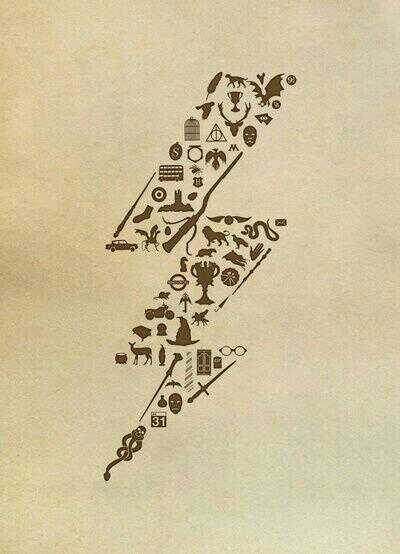
\includegraphics[scale=0.3]{harrypotter}
%	\caption{Test of figure.}
%	\label{centerOfMassDiagram}
%\end{figure}


%\begin{table}[H]
%	\centering
%	\begin{tabular}{|p{4.8cm}|p{2cm}|}
%		\hline%------------------------------------------------------------------------------------
%		\textbf{Characteristics}                 &  \textbf{Value} \unitWh{Unit}  \\
%		\hline%------------------------------------------------------------------------------------
%		Nominal output current                   &  5 \unitWh{A}  	\\
%		\hline%------------------------------------------------------------------------------------
%		Peak current (<20 s)                     &  15 \unitWh{A}	\\
%		\hline%------------------------------------------------------------------------------------
%		Current control PWM frequency 				   &  53,6 \unitWh{kHz}  \\
%		\hline%------------------------------------------------------------------------------------
%		Sample Rate of PI current controller     &  53,6 \unitWh{kHz}  \\
%		\hline%------------------------------------------------------------------------------------
%	\end{tabular}
%	\caption{Important parameters of the motor control board.}
%	\label{MotorControlBoardTable}
%\end{table}

%\begin{flalign}
%\eq{J_F \vec{\ddot{\theta}_F}} { -B_F \vec{\dot{\theta}_F} + \vec{l_F} \times (m_F\cdot \vec{g}) + \vec{l_w} \times \vec{F} - \vec{\tau_m} + B_w \vec{\dot{\theta}_w}} \unit{N\cdot m}
%\label{frameModelEq}
%\end{flalign}

%\begin{flalign}
%\eqOne{\tau_{m}[n]}{\num{-8,314} \cdot e_{\theta}[n]+ \num{7,422} \cdot e_{\theta}[n-1] + \num{8,3023} \cdot e_{\theta}[n-2] }
%\eqTwo{ - \num{7,434} \cdot e_{\theta}[n-3] + \num{1,382} \cdot \tau_{m}[n-1] - \num{0,3415} \cdot \tau_{m}[n-2] }
%\eqThree{- \num{0,001638} \cdot \tau_{m}[n-3]} \unit{N \cdot m} 
%\label{eq:discControllerDiffEq}
%\end{flalign}

\section{Method}
\begin{itemize}
\item Model - Drawing, equations, linear equations.
\item Controller - Diagram of controller.
	\item Angle controller - include observer, linear controller.
\item Network effect on the system - Analysis of delay in the system.
\end{itemize}
\section{Results}
Simulation vs. reality. \\
%Design a setup that allows a nice measurement of reality - yet to be done\\
Comment on the results and how that correlates with reality, without discussing possible issues or improvements.

\section{Discussion}
Discussing possible issues or improvements of the above results.

\section{Conclusion}
Summary - what we want the reader to remember.
\section*{Acknowledgement}
Henrik XXXXX, associated professor at Aalborg University \\
Christoffer Sloth, associated professor at Aalborg University

% trigger a \newpage just before the given reference
% number - used to balance the columns on the last page
% adjust value as needed - may need to be readjusted if
% the document is modified later
%\IEEEtriggeratref{8}
% The "triggered" command can be changed if desired:
%\IEEEtriggercmd{\enlargethispage{-5in}}

% references section

% can use a bibliography generated by BibTeX as a .bbl file
% BibTeX documentation can be easily obtained at:
% http://mirror.ctan.org/biblio/bibtex/contrib/doc/
% The IEEEtran BibTeX style support page is at:
% http://www.michaelshell.org/tex/ieeetran/bibtex/
\bibliographystyle{IEEEtran}
% argument is your BibTeX string definitions and bibliography database(s)
%\bibliography{IEEEabrv,../bib/paper}
%
% <OR> manually copy in the resultant .bbl file
% set second argument of \begin to the number of references
% (used to reserve space for the reference number labels box)

	%\begin{thebibliography}{}	
	%%\bibitem{IEEEhowto:kopka}
	%%H.~Kopka and P.~W. Daly, \emph{A Guide to \LaTeX}, 3rd~ed.\hskip 1em plus
	%%  0.5em minus 0.4em\relax Harlow, England: Addison-Wesley, 1999.
	%
	%\end{thebibliography}

% that's all folks
\end{document}

